\documentclass[./main.tex]{subfiles}

\begin{document}

\section{Ejercicio 2: Watering Grass}
\label{sec:ej2}

\subsection{Presentación}
\label{sec:ej2-intro}

\paragraph{} El segundo ejercicio presenta el problema \textit{UVa 10382, Watering Grass}\footnote{\url{https://onlinejudge.org/index.php?option=onlinejudge&Itemid=8&page=show_problem&problem=1323}}. Que es un problema de combinatoria y minimización, buscando usar la mínima cantidad de aspersores para cubrir completamente un cuarto.

\paragraph{} El cuarto está definido como un rectángulo de largo \(l\) y ancho \(w\), con \(l, w \in \mathbb{N}_0\), y \(n\) aspersores, cada uno cubriendo un círculo de radio \(r_i\) desde la posición \((x_i, \frac{w}{2})\), con \(0 \leq x_i \leq l \in \mathbb{N}_0\). \\
\(l, w, n\), y cada \(r_i, x_i\) son datos que entran por el standard input. Y el resultado se devuelve por el standard output.

\subsection{Algoritmo}
\label{sec:ej2-algo}

\paragraph{} El problema requiere calcular el area del rectángulo que cada aspersor cubre. Pero se puede ver que de cada aspersor sólo nos importa el area rectangular entre los puntos donde interseca con el rectángulo del cuarto, ya que el area cubierta afuera sólo puede ser ocupada por el area rectangular de otro aspersor o dejaría un area sin cubrir por ningún aspersor (ver Figura \ref{fig:ej2-two-sprinklers}). \\
\indent Entonces los aspersores con radio \(r_i < \frac{w}{2}\) pueden ser ignorados, ya que no llegan a intersecar con el lado del rectángulo. Y para los aspersores que quedan se los considera no como círculos, sino como su rectángulo subyacente (ver Figura \ref{fig:ej2-simple-sprinkle}). \\
Tomamos \(izq_i\), y \(der_i\) como el lado izquierdo y derecho del rectángulo subyacente del aspersor \(i\).

\begin{figure}[H]
\centering

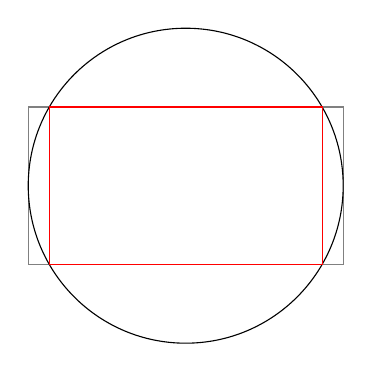
\begin{tikzpicture}
  \draw[gray] (0, 0) rectangle (4, 2);
  \draw (2, 1) circle (2);
  \draw[red] (0.2679, 0) rectangle (3.7321, 2);
\end{tikzpicture}

\caption{Marcado en rojo está el rectángulo subyacente.}
\label{fig:ej2-simple-sprinkle}
\end{figure}

\begin{figure}[H]
\centering

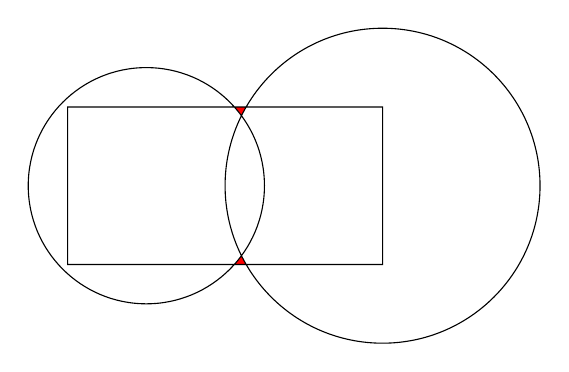
\begin{tikzpicture}
  \def\R{(0, 0) rectangle (4, 2)}
  \def\A{(1, 1) circle (1.5)}
  \def\B{(4, 1) circle (2)}

  \begin{scope} %A: Fill intersection
    \clip \R \A \B;
    \fill[red] \R;
  \end{scope}

  \begin{scope} %A: Clear intersection of circles
    \clip \A \B;
    \fill[white] \R;
  \end{scope}

  \draw \R \A \B; %A: Outline
\end{tikzpicture}

\caption{Marcada en rojo hay un ejemplo de area que ningún círculo cubre.}
\label{fig:ej2-two-sprinklers}
\end{figure}

\paragraph{} Partiendo de esa simplificación armamos un algoritmo goloso que primero ordena los aspersores según menor \(izq_i\). Y luego busca el \(i_0\) de izquierda a derecha que tenga \(izq_{i_0} \leq 0\) y que maximice la distancia entre 0 y \(der_{i_0}\), para después repetir este paso, pero buscando \(i_1\) tal que \(izq_{i_1} \leq der_{i_0}\), y maximice la distancia entre \(der_{i_0}\) y \(der_{i_1}\), y seguir tomando decisiones golosas hasta, o no haber más aspersores (caso que no se puede resolver), o haber llenado el cuarto (caso que se encontró la solución optima, ver \textbf{\ref{sec:ej2-dem} Demostración}). \\
En esencia, resolviendo subproblemas avanzando hacia cubrir todo el cuarto.

\paragraph{} Como miramos cada aspersor una vez, el algoritmo resuelve el problema en \(\bigO{n}\) pasos, aunque tiene el overhead \(\bigO{n\ log(n)}\) de ordenar los aspersores. Por lo que el problema lo resolvemos en \(\bigO{n\ log(n)}\) pasos.

\subsection{Demostración}
\label{sec:ej2-dem}

\paragraph{} Para la demostración planteamos:
\begin{itemize}
  \item A \(\mathcal{S}\) el espacio de soluciones. Con \(S = s_1, \ldots, s_m \in \mathcal{S} \mid izq_{s_1} \leq 0 \land der_{s_m} \geq l \land der_{s_i} \leq izq_{s_{i+1}}\). \\
  Se puede ver que para una instancia del problema, todas las soluciones \(S \in \mathcal{S}\) tienen el mismo largo, ya que para ser solución tienen que minimizar su largo. 
  \item A \(G_k = g_1, \ldots, g_k\) la secuencia golosa luego de haber hecho \(k\) decisiones golosas. O sea que, \(izq_{g_1} \leq 0 \land g_{i+1} = max_j\{der_j - der_{g_i} \mid der_{g_i} \leq izq_j\}\).
\end{itemize}

\paragraph{} Entonces queremos probar: \begin{itemize}
  \item[\textbf{1)}] Cualquier solución óptima \(S = s_1, \ldots, s_m\) puede ser modificada para obtener una solución óptima que use una decisión golosa.
  \item[\textbf{2)}] La secuencia \(G_k\) puede ser extendida a una solución óptima.
\end{itemize}

\paragraph{} Primero probamos \textbf{1)}, que se puede ver porque si tomamos la solución ópitma \(S = s_1, \ldots, s_{k-1}, s_k, s_{k+1}, \ldots, s_m\) y armamos \(S' = s_1, \ldots, s_{k-1}, g_k, s_{k+1}, \ldots, s_m\) tal que \(g_k = max_j\{der_j - der_{s_{k-1}} | der_{s_{k-1}} \leq izq_j\}\), \(S'\) sigue siendo una solución óptima ya que \(der_{s_{k-1}} \leq izq_{g_k}\) y \(der_{g_k} \geq der_{s_k}\) por lo que \(der_{g_k} \leq izq_{s_{k+1}}\). \\
De esta forma se puede seguir modificando a \(S\), hasta haber tomado \(m\) decisiones golosas y se llegaría a una secuencia golosa.

\paragraph{} Y ahora probamos \textbf{2)} usando el método inductivo. \begin{itemize}
  \item Definimos la proposición \(P(k) \equiv G_k\) se puede extender a una solución óptima.
  \item[\textbf{Caso base:}] \(P(0)\). Es trivial porque \(G_0 \equiv \emptyset\).
  \item[\textbf{Paso inductivo:}] \(P(k) \Rightarrow P(k+1)\). Si \(k+1 > m\) entonces es trivial, ya que \(G_k\) ya sería la solución óptima. \\
    Lo revisamos entonces para \(k+1 \leq m\). Por \textbf{HI} tenemos que \(G_k = g_1, \ldots, g_k\) es extensible a una solución \(S = g_1, \ldots, g_k, s_{k+1}, \ldots, s_m\). Como \(S\) es solución sabemos que \(der_{g_k} \leq izq_{s_{k+1}} \land izq_{s_{k+2}} \leq der_{s_{k+1}}\), por lo que si tomamos \(g_{k+1} = max_j\{der_j - der_{g_k} \mid der_{g_k} \leq izq_j\}\) se mantiene que \(der_{g_k} \leq izq_{g_{k+1}}\), y como \(der_{s_{k+1}} \leq der_{g_{k+1}}\) se mantiene que \(izq_{s_{k+2}} \leq der_{g_{k+1}}\). Por lo que \(G_{k+1}\) es extensible a una solución. \done
\end{itemize}

\end{document}
